%%%%%%%%%%%%%%%%%%%%%%%%%%%%%%%%%%%%%%%%%%%%%%%%%%%%%%%%%%%%%%%%%%%%%%%%%%%%%%%%%%%%%%%%%%%%%%%%%%%
\chapter{Background} \label{ch:Concepts}

\section{Introduction}
\section {FMCW radars}
In order to retrieve the best data for our application we first need to understand how the radar works. The following sections will try explain how the radar calculates the range, velocity and angle of an object.
\subsection{range Detection}
An FMCW radar transmits a signal called a “chirp”. A chirp is a sinusoid whose frequency  increases linearly with time.
%% put A t and f t plot
A chirp is characterized by a start frequency (fc), bandwidth(B) and duration (Tc). The slope (S) of the chirp is the rate at witch the frequency of the chirp increases and is given by:
\begin{equation}
    S=\frac{B}{T_c}
\end{equation}
%%PUT SOME TEXT
Object detection follows this steps:
\begin{enumerate}
    \item The chirp is transmitted by the TX antenna
    \item The chirp is reflected off an object and the reflected chirp is received at the RX antenna
    \item The RX signal and TX signal are ‘mixed’ and the resulting signal is called an ‘IF signal’
\end{enumerate}


%%PUT IMAGE
%%%When the transmitted chirp encounters an object it will reflect back to the radar and will be captured by the RX antenna.
The RX signal is a sum of delayed versions of the TX signal. This means that the resulting IF signal will be a combination of sinusoids. Each of this correspond to a reflection of an object. For object $i$ the corresponding frequency $f_i$ is equal to:
\begin{equation}
    f_i=S\tau_i
\end{equation}
Where $\tau_i$ is equal to the round trip delay of the wave and is equal to:
\begin{equation}
    \tau_i=\frac{2d_i}{c}
\end{equation}
Where $d_i$ corresponds to the distance of the object to the radar and $c$ the speed of light.
%% PUT image
Putting this together the distance of object $i$ is given by:
\begin{equation}
    d_i=\frac{f_ic}{2S}
\end{equation}
\subsection{range resolution}
\subsection{velocity Detection}
\subsection{angle Detection}

 %A cluster is just a subset of points of the cloud that are close together. This takes into account if a point has alot of close neighbours. If it has than it is considered a cluster.  
- New Technology
- New possibilities
\section {ROS}
Robot Operating System (ROS) is an open-source, meta-operating system that provides libraries and tools to help developers create robotic applications. This includes hardware abstraction, device drivers, tools for introspection, message-passing and more.
\subsection{ROS architecture}
%MORE STUFF
The ROS structure is composed by:
\begin{itemize}
\item \textbf{Nodes} - Processes that perform computation.
\item \textbf{Messages} - ROS predefined data type used to communicate between nodes. 
\item \textbf{Topics} - Nodes can send messages by publishing to a topic or receive them by subscribing to a topic. 
\item \textbf{Master} - Provides registration of names (helps nodes find each other).
% V
\item \textbf{rosout} - ROS equivalent of stdout 
\item \textbf{roscore} - Master+rosout+parameter server. 
%X
\end{itemize}

%%REVER ISTO

Figure \ref{fig:ros_concepts} shows an overview of the general architecture of ROS.

\begin{figure}[h] 
\centerline{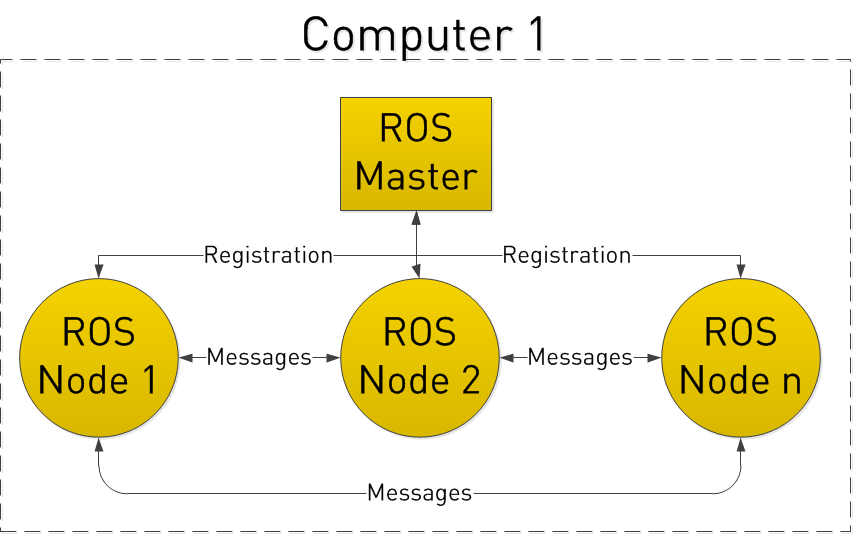
\includegraphics [width=0.5 \textwidth]{imgs/chapter2/rosgraph.png}}
\caption{Examples of 2D image filters (from \cite{baranov2014}).}
\label{fig:exemploskernel}
\end{figure}
\section {Navigation}
\subsection{Mapping}
gmapping, slam, eurico
\subsection{Localization}
AMCL
\subsection{Path Planning}
dijaktra A*



This chapter introduces the main concepts and topics involved in this dissertation's work. Firstly, there is a brief discussion about drones and their usages in today's landscape. \cite{uavhist} \ac{UAV}s
\begin{description}
    \item[Agriculture] Estimate harvest volumes using digital images collected by \ac{UAV}s\cite{harvest}. Crop monitorization, analyses and protection\cite{crop}\cite{analyses}.  
\end{description}

\section{Drones} 



\begin{table}[ht]
	\center
	\caption{Types of \ac{UAV}s and corresponding features (adapted from \cite{UAVtable}).}
	\label{tab:dronetypes}
	\begin{adjustbox}{width={\textwidth}}
    \begin{tabular}{|l|l|l|l|}
    \hline
    \textbf{} & \textbf{Pros} & \textbf{Cons} & \textbf{Typical Uses} \\ \hline
    \textbf{Multi-Rotor}      & \begin{tabular}[c]{@{}l@{}}$\bullet$ Accessibility \\ $\bullet$ Ease of use \\$\bullet$ \ac{VTOL}\\ and hover flight \\$\bullet$ Good camera control \\$\bullet$ Can operate in a confined area \end{tabular} & \begin{tabular}[c]{@{}l@{}}$\bullet$ Short flight times  \\ $\bullet$ Small payload capacity  \end{tabular}   & \begin{tabular}[c]{@{}l@{}}$\bullet$ Aerial photography and video \\ $\bullet$ Aerial inspection \end{tabular}  \\ \hline
    \textbf{Fixed-Wing}      & \begin{tabular}[c]{@{}l@{}}$\bullet$ Long endurance \\ $\bullet$ Large area of coverage \\$\bullet$ Fast flight speed \end{tabular} & \begin{tabular}[c]{@{}l@{}}$\bullet$ Requires take-off and landing area  \\ $\bullet$ No \ac{VTOL}/hover \\ $\bullet$ Harder to fly, more training required \\ $\bullet$ Expensive  \end{tabular}   & \begin{tabular}[c]{@{}l@{}}$\bullet$ Aerial mapping \\ $\bullet$ Pipeline and Power line inspection \end{tabular}  \\ \hline
    \textbf{Single-Rotor}      & \begin{tabular}[c]{@{}l@{}}$\bullet$ VTOL and hover flight \\ $\bullet$ Long endurance \\$\bullet$ Heavier payload capability \end{tabular} & \begin{tabular}[c]{@{}l@{}}$\bullet$ Less reliable  \\ $\bullet$ No \ac{VTOL}/hover \\ $\bullet$ Harder to fly, more training required \\ $\bullet$ Expensive  \end{tabular}   & \begin{tabular}[c]{@{}l@{}}$\bullet$ Aerial LIDAR laser scanning \\ $\bullet$ Pipeline and Power line inspection \end{tabular}  \\ \hline
\end{tabular}
\end{adjustbox}
\label{tab:tabelauav}
\end{table}
     

\section{Image Processing }  


Figure \ref{fig:history} shows a brief overview of the most significant advances in the field of computer vision over the last few decades.  


\begin{figure}[h] 
\centerline{\includegraphics [width=0.8 \textwidth]{imgs/chapter2/history}}
\caption{A timeline overview of some of the most active topics of research in computer
vision (from \cite{livro}).}
\label{fig:history}
\end{figure}


\subsection{Background}


One of the most sought-after goals in the field of computer vision is the analysis of a given image and recognizing and labelling all of the objects present in said input image. 

\begin{figure}[h] 
\centerline{\includegraphics [width=0.8 \textwidth]{imgs/chapter2/yoloDog}}
\caption{Example of Object Detection (from \cite{yoloDog}).}
\label{fig:yoloDog}
\end{figure}






\subsection{ImageNet challenge}




\subsection{Deep Neural Networks}


 The output $\mathbf{y}$ is obtained by applying an activation function to the weighted sum between inputs and their associated weights, and is expressed in Equation \ref{eq:eqneuron}:  

\begin{equation}\label{eq:eqneuron}
    y = f(\xi) = f(\sum_{i=1}^{n} x_i.w_i + \theta)
\end{equation}


\subsubsection{Convolutional Neural Networks}


\begin{equation}\label{eqn:1}
f[m,n] \circledast g[m,n] = \sum_{i=-{\infty}}^{\infty} \sum_{j=-{\infty}}^{\infty} f[i,j] . g[m-i,n-j]
\end{equation}


\begin{figure}[h] 
\centerline{\includegraphics [width=1 \textwidth]{imgs/chapter2/exemploskernel}}
\caption{Examples of 2D image filters (adapted from \cite{masterkernel}).}
\label{fig:exemploskernel}
\end{figure}





\begin{description}

 \item[Input Layer] Composed of the raw pixel data from the image (usually a 3 dimension matrix corresponding to the three color channels R,G,B).
 
\end{description}


A simple overview of a \ac{CNN} is shown in Figure \ref{fig:sampleCNN}.


\begin{figure}[h] 
\centerline{\includegraphics [width=1 \textwidth]{imgs/chapter2/samplecnn}}
\caption{ Example of a Convolutional Neural Network  (from \cite{tese}).}
\label{fig:sampleCNN}
\end{figure}

The Network receives an input image (3 dimensional vector: width, height, channels). This input is then transformed through a set of hidden layers, changing the shape and size of the original data to obtain an output vector consisting of each class scored according to the level of certainty that said class is present in the input image.  


%\begin{figure}[H] 
%\centerline{\includegraphics [width=0.8 \textwidth]{imgs/chapter2/Krizhevsky}}
%\caption{ Example of a Convolutional Neural Network Architecture (from %\cite{Krizhevsky}).}
%\label{fig:Example_object_det}
%\end{figure}


Each layer has an input volume and outputs a certain volume to the next layer. The size of each output volume is dependent on the layers' hyperparameters:


\begin{description}

 \item[Depth] This first parameter corresponds to the number of filters present in layer. These filters have different goals, each producing different feature maps. They can be used to detect edges, gradients, downsample the input... 


 
\end{description}


\subsection{Examples of Convolutional Networks}

$ f: {\rm I\!R}^{N} \rightarrow \{-1,+1\}$, 

\section{Evaluation of Object Detection Algorithms}

\begin{description}

 \item[\ac{TP}] True positives represent the instances where the predicted class is equal to the actual class present in the image.

\end{description}

